\section{Этапы проектирования конструкции РЭС и их характеристика}

Во время работы в малом предприятии трудно заметить
четкие границы перехода между этапами конструирования РЭС,
так как процесс разработки, кроме того, что увлекателен сам по себе,
в данном случае, ещё и не усложнён бюрократической волакито.

Существует, по крайней мере, два способа
провести разделение процесса проектирования
на этапы:

\begin{enumerate}
\item По стадиям разработки конструкторской документации;
\item По стадиям работы в САПР.
\end{enumerate}

Обычно,
в технической литературе, приводится минимум пять стадий
разработки
конструкторской документации ~\cite{Rotkop1976}.

Эти стадии включают в себя:

\begin{enumerate}
\item Техническое задание
\item Техническое предложение
\item Эскизный проект
\item Технический проект
\item Выпуск рабочей документации
\end{enumerate}

Техничское задание я получил в устном виде от работников отдела.

Техническим предложением можно считать
исходную схему из журнала «Радио Лоцман».

Эскизный тогда это моя принципиальная схема и определенный в \textit{KiCAD}
формфактор платы.

Техничский проект это получившаяся в результате трассировки печатная плата.

Тогда выпуском рабочей документации — это переделанная,
в результате правок от отдела производства,
принципиальная схема и печатная плата.

Стадии работы в САПР, я бы описал следующим образом:
\begin{enumerate}
\item Создание библиотеки схемных элементов и библиотеки посадочных мест.
\item Создании принципиальной схемы со связями между элементами.
\item Верификация принципиальной схемы \textit{ERC}
  и экспорт связей в часть САПР, предназначенную для трассировки
  % Electric Rule Checker.
\item Трассировка печатной платы и верификация правил  \textit{DRC}.
  % Design Rule Checker
\end{enumerate}

Первый этап работы в САПР мною был пропущен,
по той причине, что kicad обладает большой встроенной
библиотекой посадочных мест.

% Сюда скриншот окна со встроенной библиотейкой посадочных мест

\begin{figure}[H]
  \centering
  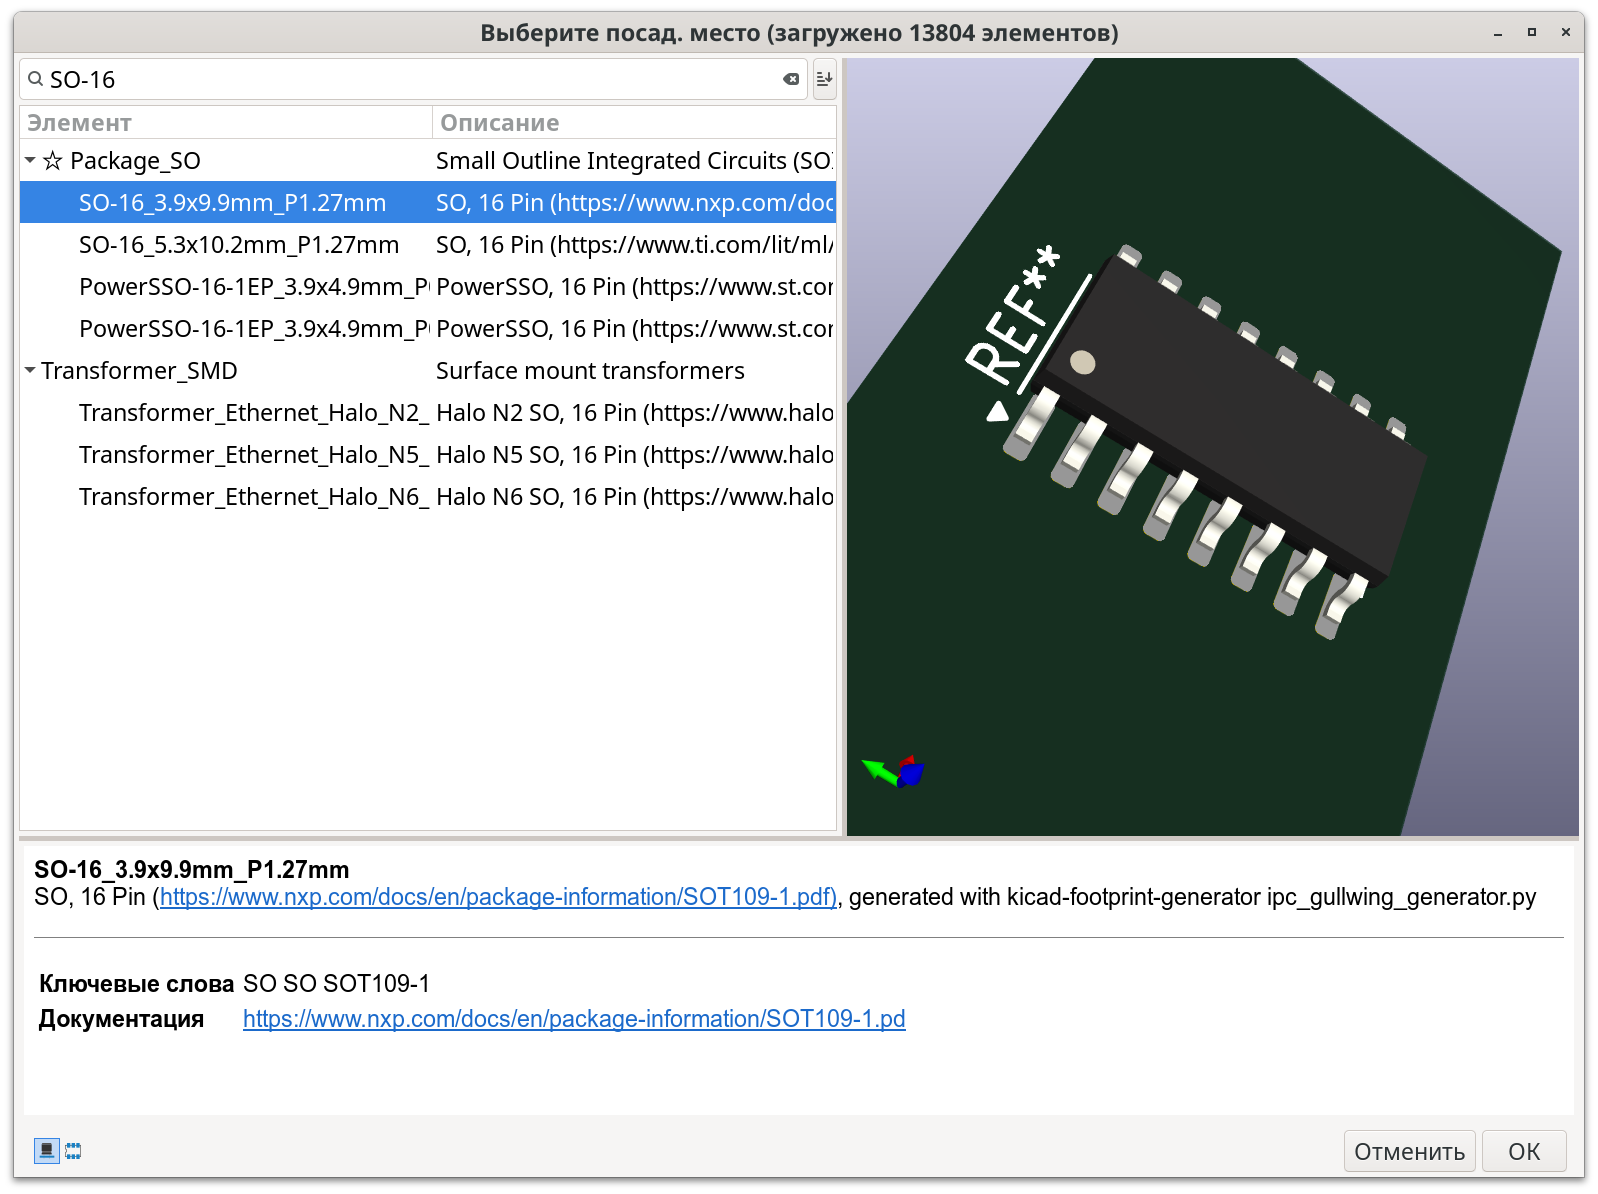
\includegraphics[scale=0.2]{kicad-so-package-footprint-with-3d.png}
  \caption{Снимок экрана с меню выбора посадочных мест в \textit{kicad-pcbdoc}}
\end{figure}

Также была использована готовая
схемная библиотека, выполненная в рамках стандартных УГО. 
% https://github.com/KiCad-RU/kicad-symbols-gost

% Скриншот окна со схемной библиотекой по ГОСТ
\begin{figure}[H]
  \centering
  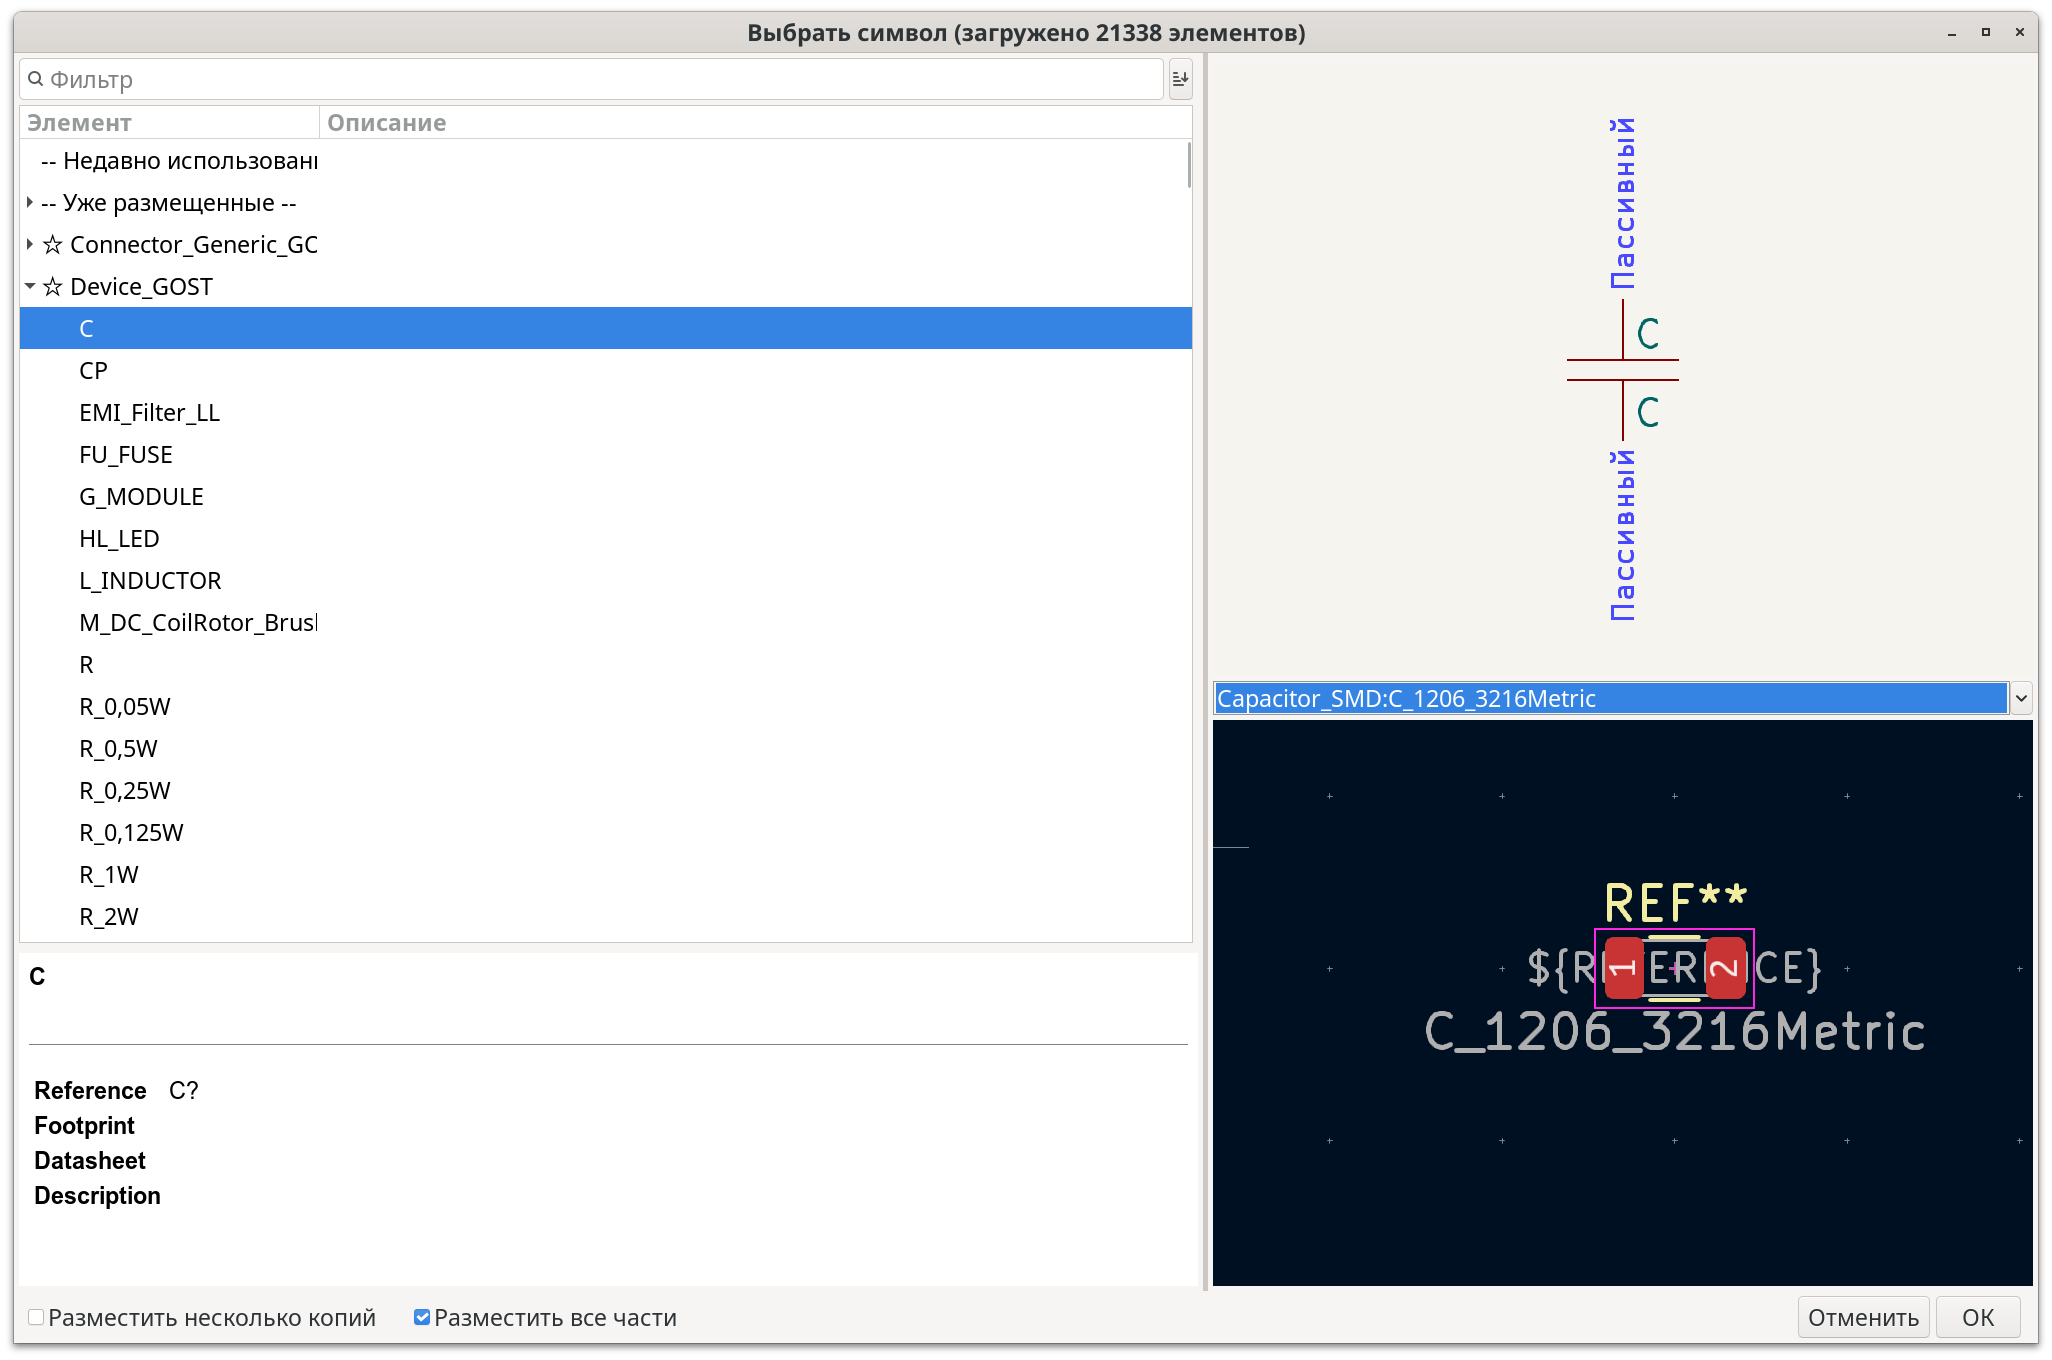
\includegraphics[scale=0.2]{kicad-capacitor-gost-library.png}
  \caption{Снимок экрана с меню выбора cхемных компонентов
    мест в \textit{kicad-eeschema}}
\end{figure}


После долгой работы над схемой, её верификация \textit{ERC}
не показывала предупреждений о нарушении.

Спустя несколько дней к такому же результату,
я пришел выполняя верификацию разведённой печатной платы \textit{DRC}.

Однако верификация не уберегла,
от ошибки:

Неправильного включения транзистора на принципиальной схеме.

Помочь могло либо внимание к сложным местам,
потому что именно место, где я допустил ошибку,
изначально казалось самым сложным, как в создании схемы,
так и в трассировке платы. Либо использования специальной САПР симулятора.

\newpage

% Local Variables:
% compile-command: "sh build.sh"
% End:
